\chapter{Analisi dei Risultati} 

I dati relativi agli indici di prestazione di interesse (tempi di risposta e throughput) misurati 
nelle precedenti fasi di test sono stati in seguito aggregati e visualizzati in forma di grafici. 
Infatti, in base al tipo di test effettuato, tali grafici si suddividono in due categorie: i grafici di 
throughput e tempi di risposta del sistema in stato di instabilit\`a (front server sovraccarico) e 
quelli relativi al sistema in condizione di stazionariet\`a (front server non sovraccarico), ovvero quelli gestiti
attraverso il meccanismo di overload management.

\section{Sistema senza Overload Management}

\subsection{Response Time}

In questo scenario l'utilizzazione del front-end server \'e praticamente uguale a 1, perci\`o 
non riesce a completare tutte le richieste entranti, con la inevitabile 
situazione di veder aumentare indefinitamente la lunghezza della sua coda. Di 
conseguenza il tempo di risposta del sistema tende a divergere all'aumentare del tempo di 
simulazione. Il grafico illustrato di seguito mostra tale scenario:

\begin{figure}[H]
 \centering
 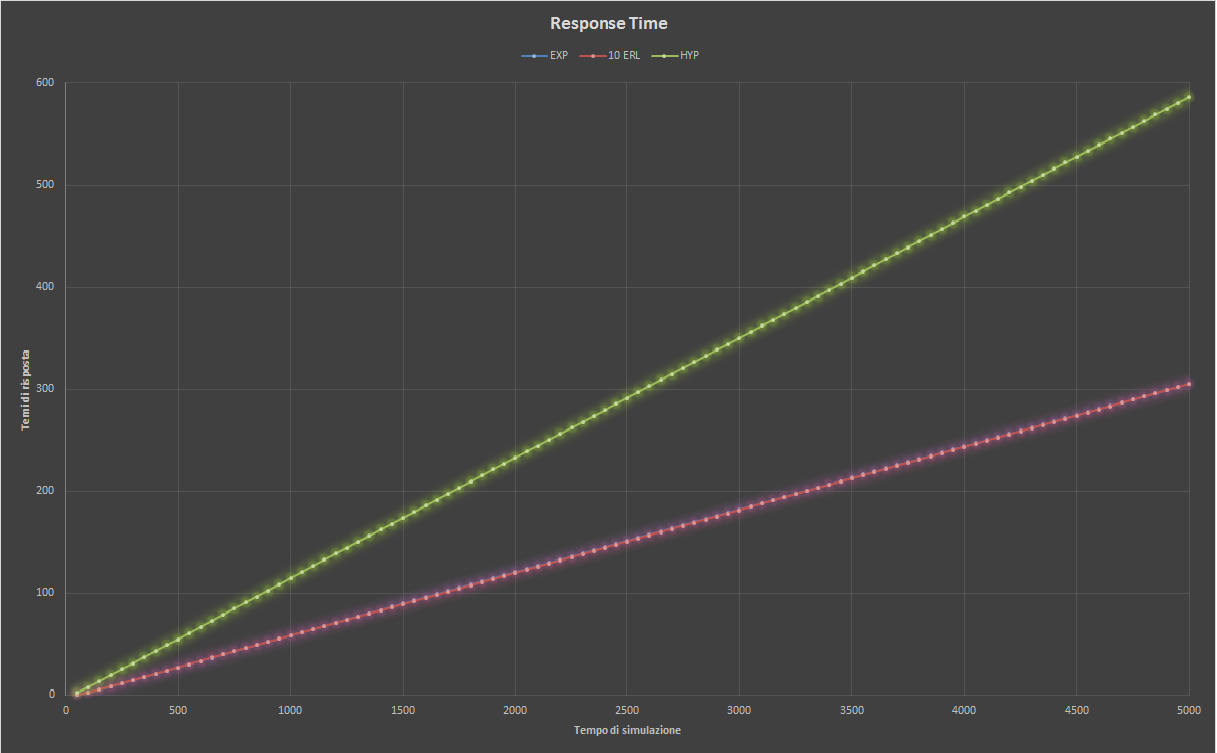
\includegraphics[scale=0.45]{img/responseTime.png}
 \caption[Tempi di risposta del sistema instabile]{Tempi di risposta del sistema instabile}
 \label{fig:Tempi di risposta del sistema instabile}
\end{figure}

Come si intuisce dal grafico sopra riportato, i tempi di risposta si contraddistinguono in base
al tipo di distribuzione dei tempi di servizio del front-end server (iperesponenziale, 10-erlang 
ed esponenziale), e in base all'andamento delle curve dei tempi di risposta, risulta evidente 
come la distribuzione iperesponenziale dei tempi di servizio del front-end risulta peggiore 
che nel caso esponenziale e 10-erlang, dove i tempi rimangono uguali.

Questa sostanziale differenza \`e dovuta al fatto che, nel caso iperesponenziale, avendo 
preimpostato la probabilità \textbf{p=0.1}, la varianza dei tempi di servizio delle richieste risulta 
essere molto elevato con la conseguenza di rallentare notevolmente il front-end server.
Di conseguenza la curva dei tempi di risposta della iper-esponenziale diverge pi\`u 
rapidamente rispetto alle controparti 10-erlang ed esponenziale. Tuttavia il grafico mostra 
anche un aspetto insolito: la curva del tempo di risposta della 10-erlang coincide 
praticamente con la curva dell'esponenziale anche avendo impostato un parametro K=10, 
mentre ci si aspettava, al contrario, un miglioramento dei tempi di risposta rispetto alla curva 
della esponenziale. Probabilmente la scelta del parametro K pari a 10 \'e insufficiente a 
garantire un miglioramento significativo.

\subsection{Autocorrelazione}

L'evidente divergenza dei tempi di risposta del sistema \'e evidenziata anche dalla forte 
correlazione presente dai tempi di risposta delle singole richieste presenti nel sistema. Il 
grafico seguente illustra tale correlazione sulle tre distribuzioni:

\begin{figure}[H]
 \centering
 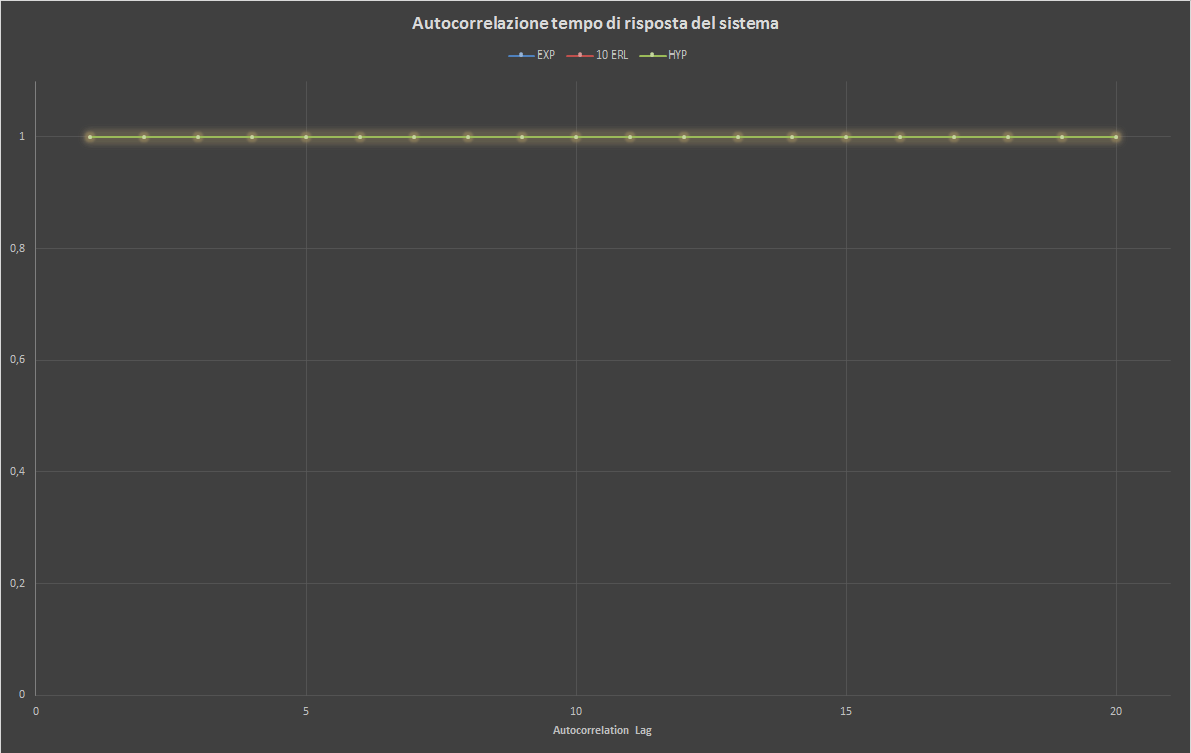
\includegraphics[scale=0.45]{img/autocorrelation.png}
 \caption[Autocorrelazione dei tempi di risposta]{Autocorrelazione dei tempi di risposta}
 \label{fig:Autocorrelazione dei tempi di risposta}
\end{figure}

Dal grafico non si evince bene ma i valori dell'autocorrelazione relativi alla distribuzione
iperesponenziale sono leggermente inferiori rispetto agli altri due casi (nell'ordine di $10^{-2}$)
ma si assestano tutti nell'intorno di 0.9.

\subsection{Useful Throughtput}

Il grafico successivo mostra l'andamento dello useful throughput i cui valori sono stati
misurati dagli stessi test usati per il tempo di risposta del sistema. Anche in questo caso si 
distinguono le diverse distribuzioni dei tempi di servizio del front-end server:

\begin{figure}[H]
 \centering
 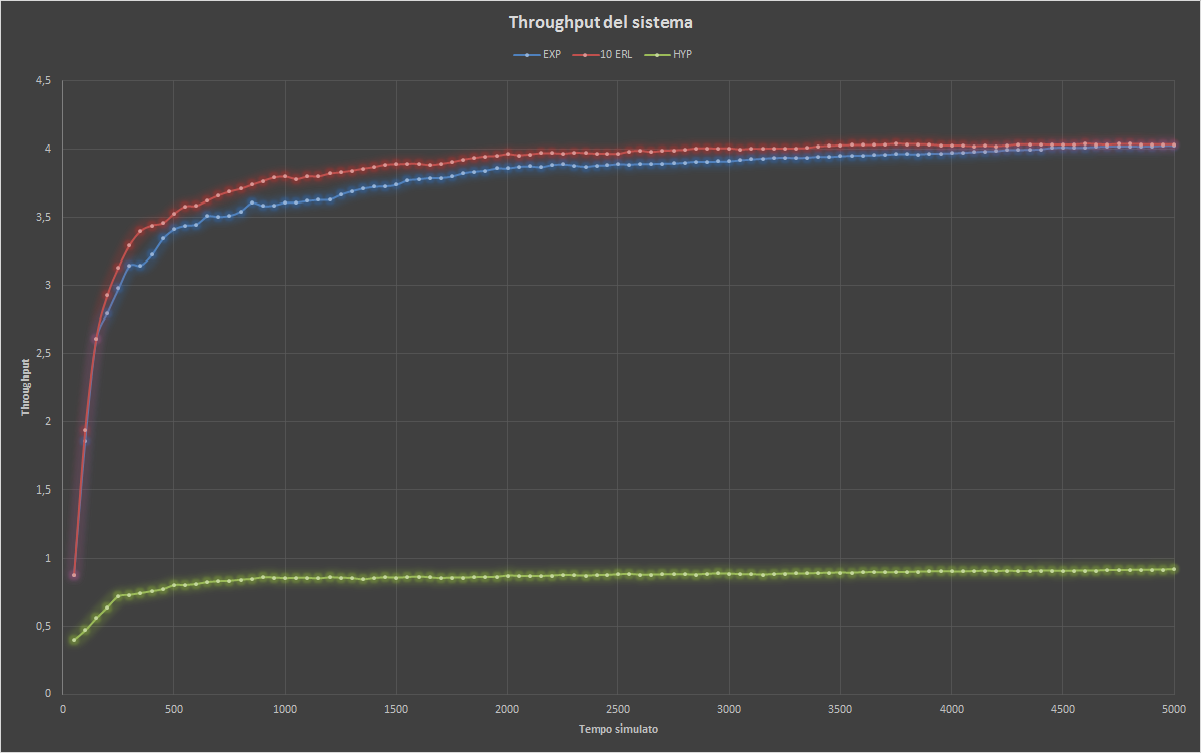
\includegraphics[scale=0.45]{img/throughput.png}
 \caption[Throughput del sistema instabile]{Throughput del sistema instabile}
 \label{fig:Throughput del sistema instabile}
\end{figure}

Anche in questo caso si nota la notevole differenza dello useful throughput  del caso 
iperesponenziale da quelli esponenziali e 10-erlang, i quali coincidono per valori di run  
simulativi molto alti.
Lo useful throughput \'e l'unico indice di prestazione che presenta un andamento stazionario 
all'aumentare del tempo di simulazione. Si pu\`o notare dal grafico, infatti, che tale valore di 
stazionariet\`a \'e all'incirca pari a 4 sessioni completate per unit\`a di tempo.


Di seguito sono stati riportati gli intervalli di confidenza stimati per ogni distribuzione. 
\begin{itemize}
 \item \textit{\textbf{Esponenziale}} : $[ 3,66109876 ; 3,83534225 ]$
 \item \textit{\textbf{10 Erlang}} : $[ 3,75592814 ; 3,92657294 ]$
 \item \textit{\textbf{Iperesponenziale}} : $[ 0,84149673 ; 0,87406350 ]$
\end{itemize}

Infine viene riportato l'istogramma relativo allo useful throughput dato che l'unico
indice con comportamento steady-state:

\begin{figure}[H]
 \centering
 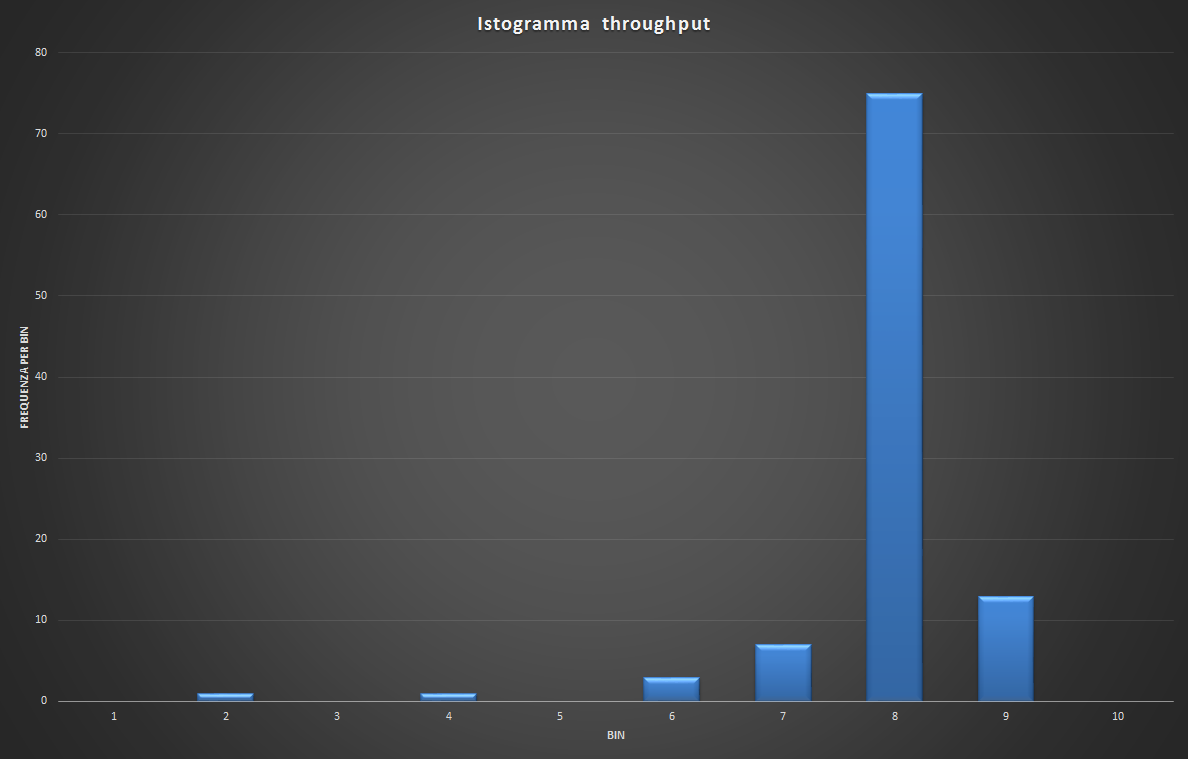
\includegraphics[scale=0.45]{img/istogramma.png}
 \caption[Istogramma del throughtput]{Istogramma del throughtput}
 \label{fig:Istogramma del throughtput}
\end{figure}




\section{Sistema con Overload Management}

\subsection{Response Time}

\subsection{Autocorrelazione}

\subsection{Useful Throughtput}

\subsection{Drop e Aborted Ratio}